%Template by Mark Jervelund - 2015 - mjerv15@student.sdu.dk

\documentclass[a4paper,10pt,titlepage]{report}

\usepackage[T1]{fontenc}
\usepackage[english]{babel}
\usepackage{graphicx}
\usepackage{fancyhdr}
\usepackage{lastpage}
\usepackage{listings}
\usepackage{marvosym}
\usepackage[document]{ragged2e}
\usepackage[margin=1in]{geometry}
\usepackage{color}
\usepackage{datenumber}
\usepackage{venndiagram}
\usepackage{chngcntr}
\usepackage[utf8]{inputenc}
\usepackage{amsmath,amsthm}
\usepackage{mathtools}
\usepackage{wrapfig}
\usepackage{multirow}
\usepackage[
    backend=biber,
    style=numeric,
    sorting=ynt
]{biblatex}

\newtheorem{theorem}{Theorem}



\addbibresource{bibliography.bib}


\DeclarePairedDelimiter\norm\lVert\rVert
\setdatetoday
\addtocounter{datenumber}{0} %date for dilierry standard is today
\setdatebynumber{\thedatenumber}
\date{}
\setcounter{secnumdepth}{0}
\pagestyle{fancy}
\fancyhf{}
\title{Masters Thesis}

\newcommand{\Z}{\mathbb{Z}}
\lhead{Masters Thesis}
\rhead{Mark Jervelund}
\rfoot{Page  \thepage \, of \pageref{LastPage}}
\counterwithin*{equation}{section}

\begin{document}
    \begin{titlepage}
        \centering
        \vspace*{9\baselineskip}
        \huge
        \bfseries
        Jepsen methods usage for ACID compliance in Hyperscale Cloud Frameworks \\
        \normalfont
        Mark Jervelund \\
        Mark@jervelund.com \\
        \vspace*{9\baselineskip}
        \normalfont
        \includegraphics[scale=1]{logos/SDU_BLACK.png}
        \vfill\
        \vspace{5mm}
        Institute Of Mathematics and Computer Science, SDU \\

        %Date
        \textbf{\datedate} \\[2\baselineskip]
    \end{titlepage}

    \renewcommand{\thepage}{\roman{page}}% Roman numerals for page counter
    \tableofcontents
    \newpage
    \setcounter{page}{1}
    \renewcommand{\thepage}{\arabic{page}}


    \section*{Abstract}

    Databases allow modern society to store, manage and distribute data at a previously unprecedented scale. Having data is standard practice for most businesses. Still, it is often done monotonically on a single node, where modern needs require more storage, latency, availability, and higher performance than current systems allow. Distributing a data store in a manner that scales performance, storage, availability, and desired properties is no easy feat. In this thesis, I will present methods of verifying these properties, and I will investigate how different frameworks solve this issue or often work around the issue in a way that aligns with the requirements of the systems. \\
    \vspace{5mm}

    Within the thesis framework, I will present methods of verifying the ACID properties, how they were solved in the past compared to how they are solved today, and what trade-offs some systems have made. I will also analyze modern database use cases and whether they require the ACID properties to solve issues.\\
    \vspace{5mm}

    %TODO Summarize the findings and try to say why the thesis is worth reading.}


    \chapter{Introduction}
    Highly Distributed systems are becoming commonplace as the world grows increasingly interconnected, faster-paced, more data-driven with higher expectations of user services and products. In these situations, the end-user expects reliability, availability combined with low- latency and cost. How do we guarantee this is a distributed system that spans the planet? Is it even possible to get both consistency and availability, and is it needed in most use cases?\\
    \vspace{5mm}


    Most people are familiar with how YouTube, Facebook, Google, and Reddit behave and the quirks they sometimes present. Some users remember the YouTube video counter that got stuck at around 300 views and didn't update for a while. YouTube induced the reason it got stuck; however, it did not induce the number it got stuck on; the system was designed to stop after the counter reached 300, but the counter would often go higher. This is an example of the system not being entirely consistent; most nodes were in the correct state of stopping the count when the number got larger than 300; however other nodes weren't consistent. Therefore the servers still counted the views onto the displayed counter even though they were supposed to have been sent to a different table that verified the views before considering them legitimate. Even though the number is still not consistent worldwide, the issue of a comment or view being a few seconds or ½ a minute delayed isn't something we notice or care about.

    Many user-facing services aren't required to be ACID compliant; however, there are use cases where not being compliant can have a severe impact. Strong ACID transactions are of utmost importance when dealing with data produced and consumed in real-time, such as financial data, automated or autonomous systems, and other areas.

    These mentioned use cases are where a lack of consistency would result in loss of life or significant loss of revenue. These situations require that no matter which server we are querying, it supplies the most recent data. If we receive stale data, we are at risk of making an illegal transaction or an autonomous system making a wrong decision. This could be an automated trading system fetching stale data and making the wrong transaction, a bank withdrawal that might be overdrawing the users' accounts, or autonomous vehicles that might make decisions with stale data that can lead to fatal accidents. \\

    \vspace{5mm}
    How do we test and verify a given system's ACID compliance level? To understand this, we need to first be familiar with the basis of the consistency levels and the intended behavior and anomalies they exhibit.\\


    First, I will present ACID \& Base, their constraints, faults in database systems, how they manifest themselves, the underlying causes, and the limits that ACID properties impose on a given system. Base will be introduced to explain what relaxations are introduced to a system to gain desired properties and trade-offs.\\
    \vspace{5mm}

    Then, I will introduce Jepsen, a Clojure framework\cite{jepsonio} developed by K. Kingsbury that allows for testing distributed systems. This is done by building a directed serialization graph (DSG) via querying the target system with carefully chosen queries for traceability and recoverability.  \\
    \vspace{5mm}

    Next, I will introduce Azure Service Fabric(SF). SF is a distributed container orchestration system made by Microsoft that allows for hosting services or containers. It includes a few different built-in subsystems, but the primary interest here lies in the aspect of SF's reliable containers and the claims Microsoft makes concerning the behavior of this datastore.\\
    \vspace{5mm}

    Afterward, I will present what modern database systems promise, the ACID properties they follow, the ones they relax or disregard, and the gain and trade-offs they suffer. Here the main focus will be on Service Fabric.\\
    \vspace{5mm}

    Subsequently,  I will demonstrate the attempt to implement and execute a Jepsen test against Service Fabrics reliable containers and compare these results to Microsoft's claims.\\
    \vspace{5mm}

    Finally, I will present the way ACID properties compare to modern use cases of databases. Do we need to follow them strictly, or can we disregard them in some use cases? What are the exceptions, and what is there to gain?\\


    \chapter{Database transaction models}

    Database and data store models can be categorized into two main groups, ACID and BASE,  consistent or available.

    The underlying reason for consistency limitations is caused by the latency between nodes in the system resulting from the speed of light; in turn, systems cannot instantly distribute data between nodes. A system's availability limitation is due to the compute performance of a given system, where the solution is to either build faster servers or use more servers. Which again, both solutions have their limitations. Both models of designing the systems have their trade-offs which will be presented in this chapter.


    \section{ACID}
    The ACID Model of handling database transactions is considered monolithic by some. However, it still serves a vital and critical function for handling critical systems that require atomicity, consistency across the entire database, as well as reliability, and durability during hardware failure.\\
    \vspace{5mm}
    The ACID acronym is defined as follows in the DBMS book\cite{DBMSbook}.

    \begin{itemize}
        \item "A" stands for "atomicity," the all-or-nothing execution of transactions.
        \item "C" stands for "consistency." All databases have consistency constraints or expectations about relationships among data elements (e.g., account balances may not be negative after a transaction is finished). Transactions are expected to preserve the consistency of the database.
        \item "I" stands for "isolation," the fact that each transaction must appear to be executed as if no other transaction is executed at the same time.
        \item "D" stands for "durability," the condition that the effect on the database of a transaction must never be lost once the transaction has been completed.
    \end{itemize}

    ACID, therefore, offers strong consistency with rigorous handling of transaction isolation that prevents inaccurate data. This allows for designing a system where we can avoid operations on stale data, data loss, or "illegal" transactions. These faults will be presented further down in the paper.


    \section{BASE}
    The BASE model allows the designing of a system where we value availability, throughput, and scale-ability. This can cause issues with stale data, dirty reads, overwriting data, and other undesired behavior. This can benefit some applications where overwriting old data isn't an issue, or the newest data version might not be required as long as it eventually comes. These databases are hugely beneficial for social media, logging, and other hyper-scale systems where consistency isn't needed.\\
    \vspace{5mm}
    The Base Acronym was defined by Eric Brewer\cite{brewer2000towards} as follows:

    \begin{itemize}
        \item Basically Available – Rather than enforcing immediate consistency, BASE-modelled NoSQL databases will ensure data availability by spreading and replicating it across the database cluster nodes.
        \item Soft State – Due to the lack of immediate consistency, data values may change over time. The BASE model breaks off with the concept of a database that enforces its consistency, delegating that responsibility to developers.
        \item Eventually Consistent – The fact that BASE does not enforce immediate consistency does not mean that it never achieves it. However, until it does, data reads are still possible (even though they might not reflect the reality).
    \end{itemize}

    The BASE model of databases often has a weak consistency where stale data is considered "OK" while offering a best-effort approach with approximate answers. It gains availability, performance, and it can be viewed as a relaxed way of handling the database side of things where the system database system is simpler and easier to modify the schema.


    \section{CAP theorem}

    Eric Brewer defined the CAP Theorem\cite{CAP}. It states that a distributed database system can't provide Consistency, Availability, and Partition Tolerance in a single system. Only two of these guarantees can be met.\\
    \vspace{5mm}
    It should be noted that the definitions of the terms differ from the definitions in ACID. They are all critical when it comes to distributed systems and their behaviors. Firstly, consistency in ACID is defined as constraints on the data. By the CAP consistency concept, ACID would follow sequential consistency as defined by Lamport\cite{lamport1993how}: "the program behaves as if the memory accesses of all processes were interleaved and then executed sequentially." While the consistency in CAP is defined as Atomic Consistency (also called linearizability), it is sequential with a added constraint of real-time ordering: "Unlike sequential consistency, linearizability implicitly assumes the notion of an observable global time across all processes. Operations are modeled by an interval consisting of the period of time between the invokation and response for the operation. Each operation is assumed to take effect instantaneously at some point within this interval". \cite{CSL-TR-95-685}
    \vspace{5mm}
    CAP states we can only have two of the three properties in any given data-share system. The three different options will be explained below.


    \begin{itemize}
        \item Consistency and Partition tolerance(CP) \\ A system that delivers Consistency and Partition tolerance but the trade-off here is Availability. If a partition occurs in the system, the non-consistent nodes would have to be shut down or made unavailable to deliver consistent data. CP would cover majority protocols and most distributed databases. An example of a CP database would be MongoDB and Service Fabrics Reliable collections. These work by having partitions that contain a master and a set of replicates. The replicates simply follow the master's transaction log and apply it to their own data set. If the primary becomes unavailable, the Replicate with the most recent transaction log becomes the new master. During this switch, the partition becomes unavailable while the replicates catch up to the new master. This causes the network to remain consistent but limits availability. \\

        \item Availability and Partition tolerance (AP). If a system foregoes Consistency and delivers Availability and Partition tolerance,then in the case of a network partition between nodes, we keep serving from all nodes, but the system will serve stale data. it can also occur that rows contain different values due to multiple write operations on the different nodes. An example of an AP database would be Cassandra, where the CP has a master/replicate architecture. This would cover DNS, Caching systems. Cassandra uses a leaderless architecture; it does mean that there are multiple points of failure rather than a single one. It can be available and partition tolerant but consistency isn't guaranteed as nodes are always available and in case of partitioning the nodes will diverge while partitioned due to it's Last Write Wins model, and will later then first regain consistency once network is healed. \\

        \item Availability and Consistency (CA) \\ Database delivers consistency and availability but doesn't allow for partitions of the network or nodes. This results in a single node or single cluster system as any system distribution introduces network instability and latency that would break the system. In this case, it would cover single-node/site databases and cluster databases as well as file systems as we, in practice, wouldn't have a distributed system that doesn't allow for partitioning as it would be unusable. But an example of this would be a single node database. PostgresSQL could be an example here; however, PostgresSQL does support replication but then it becomes a CP database, which some asterisks as the system may not be consistent\cite{aphyrpostgres} as it doesn't quite behave as expected. \\
    \end{itemize}


    \newpage


    \section{Pretext to Consistency models.}

    \subsection{Availability}

    Availability refers to the gurantee a system promises doing the presence of network partitions.\cite{HighlyAvailableTransactionsVirtuesandLimitations}

    \begin{itemize}
        \item high availability:
%TODO Copy write all the below.
        \textit{
            Informally, highly available algorithms ensure “always on” operation and, as a side effect, guarantee low latency. If users of a highly available system are able to contact a (set of) server(s) in a system, they are guaranteed a response; this means servers will not need to synchronously communicate with others. If servers are partitioned from one another, they do not need to stall in order to provide clients a “safe” response to operations. This lack of fastpath coordination also means that a highly available system also provides low latency ; in a wide-area setting, clients of a highly available system need not wait for cross-datacenter communication. To properly describe whether a transactional system is highly available, we need to describe what servers a client must contact as well as what kinds of responses a server can provide, especially given the possibility of aborts. Traditionally, a system provides high availability if every user that can contact a correct (non-failing) server eventually receives a response from that server, even in the presence of arbitrary, indefinitely long network partitions between servers \cite{CAP}. As in a standard distributed database, designated servers might perform operations for different data items. A server that can handle an operation for a given data item is called a replica for that item.}\cite{HighlyAvailableTransactionsVirtuesandLimitations}
        \item Sticky Available: \textit{In addition to high availability, which allows operations on any replica, distributed algorithms often assume a model in which clients always contact the same logical replica(s) across subsequent operations, whereby each of the client’s prior operations (but not necessarily other clients’ operations) are reflected in the database state that they observe. As we will discuss in Section 5, clients can ensure continuity between operations (e.g., reading their prior updates to a data item) by maintaining affinity or “stickiness” with a server or set of servers . In a fully replicated system, where all servers are replicas for all data items, stickiness is simple: a client can maintain stickiness by contacting the same server for each of its requests. However, to stay “sticky” in a partially-replicated system,    where servers are replicas for subsets of the set of data items (which we consider in this paper), a client must maintain stickiness with a single logical copy of the database, which may consist of multiple physical servers. We say that a system provides sticky availability if, whenever a client’s transactions is executed against a copy of database state that reflects all of the client’s prior operations, it eventually receives a response, even in the presence of indefinitely long partitions (where “reflects” is dependent on semantics). A client may choose to become sticky available by acting as a server itself; for example, a client might cache its reads and writes. Any guarantee achievable in a highly available system is achievable in a sticky high availability system but not vice-versa.}\cite{HighlyAvailableTransactionsVirtuesandLimitations}
        \item transactional availability: \textit{Until now, we have considered single-object, single-operation availability. This is standard in the distributed systems literature    (e.g., distributed register models such as linearizability all concern single objects [41]), yet the database literature largely focuses on transactions: groups of multiple operations over multiple objects. Accordingly, by itself, traditional definitions of high availability are insufficient to describe availability guarantees for transactions. Additionally, given the choice of commit and abort responses— which signal transaction success or failure to a client—we must take care in defining transactional availability. We say that a transaction has replica availability if it can contact at least one replica for every item it attempts to access; this may result in “lower availability” than a non-transactional availability requirement (e.g., single-item availability). Additionally, given the possibility of system-initiated aborts, we need to ensure useful forward progress: a system can trivially guarantee clients a response by always aborting all transactions. However, this is an unsatisfactory system because nothing good (transaction commit) ever happens; we should require a liveness property .
        \vspace*{4mm}\\
        A system cannot guarantee that every transaction will commit—transactions may choose to abort themselves—but we need to make sure that the system will not indefinitely abort transactions on its own volition. We call a transaction abort due to a transaction’s own choosing (e.g., as an operation of the transaction itself or due to a would-be violation of a declared integrity constraint) an internal abort and an abort due to system implementation or operation an external abort. We say that a system provides transactional availability if, given replica availability for every data item in a transaction, the transaction eventually commits (possibly after multiple client retries) or internally aborts [9]. A system provides sticky transactional availability if, given sticky availability, a transaction eventually commits or internally aborts}\cite{HighlyAvailableTransactionsVirtuesandLimitations}

%TODO write on on Unavailable within availability the consistency models
        \item Unavailable: \textit{Not available during some types of network failures. Some or all nodes must pause operations in order to ensure safety.}
%TODO write on on Totally Available within availability the consistency models
        \item Totally Available: \textit{Available on every non-faulty node, even when the network is completely down.}


    \end{itemize}

    \subsection{Phenomena}
    %TODO Write introduction to Phenomena
    Most consistency models are defined by what Phenomena they allow or prohibit. However due to poor or loose definitions there often exist multiple different definitions on each consistency model as well as on many of the Phenomena, or simply the lack of a definitiion on some properties.

    %TODO Write Section about what ANSI defineds.

    ANSI/ISO SQL-92 [ANS92] defines the phenomena in English as follows:
    \begin{itemize}
        \item Dirty Read — Transaction T1 modifies x. Another transaction T2 then reads x before T1 commits or aborts. If T1 then aborts, T2 has read a data item that was never committed and so never really existed.
        \item Fuzzy or Non-repeatable Read — Transaction T1 reads x, and T2 modifies or deletes x and commits. If T1 then attempts to reread x, it receives a modified value or discovers that the data item has been deleted.
        \item Phantom — Transaction T1 reads a set of data items satisfying some <search condition>. Transaction T2 then creates data items that meet T1's <search condition> and commits. If T1 then repeats its read with the same <search condition>, it gets a set of data items different from the first read.
    \end{itemize}

    %TODO Write Section about what Berensonetal defineds.
    In \cite{Berensonetal} read and write skew are defined that occur due data item constraint violations. The exact definition is below: \\

    \textit{(Data Item Constraint Violation). Suppose C() is a database constraint between two data items x and y in the database. Here are two anomalies arising from constraint violation}

    \begin{itemize}
        \item
        \item \textit{Read skew Suppose transaction T1 reads x, and then a second transaction T2 updates x and y to new values and commits. If T1 reads y now, it may see an inconsistent state and therefore produce an inconsistent state as output.
        In terms of histories, we have the anomaly:  }
        A5A: r1[x]...w2[x]...w2[y]...c2...r1[y]...(c1 or a1)
        \item \textit{A5B Write Skew Suppose T1 reads x and y, which are
        consistent with C(), and then a T2 reads x and y, writes x,
            and commits. Then T1 writes y. If there were a constraint
            between x and y, it might be violated. In terms of histories:}
        A5B: r1[x]...r2[y]...w1[y]...w2[x]...(c1 and c2 occur)
        (Write Skew)
    \end{itemize}


    \begin{table}[h]
        \begin{tabular}{|l|l|l|}
            \hline
            Phenomenon                     & Anomaly Interpretation                       & Comment \\\hline
            Dirty Read                     & w1(x) ... r2(x) ... (a1 and c2 in any order) &         \\\hline
            Fuzzy Read/Non-repeatable read & r1(x) ... w2(x) ... c2 ... r1(x) ... c1      &         \\\hline
            Phantom                        & r1(P) ... w2(y in P) ... c2 ... r1(P) ... c1 &         \\ \hline
        \end{tabular}
        \caption{r:read, w:write, a:abort, c:commit}
    \end{table}


    From this knowledge a table can be made that gives us an overview of the isolation levels and what behavior and the trade-off they have.
    Isolation level Read phenomena
    Dirty read Non-repeatable read Phantom read
    read uncommitted yes yes yes
    read committed no yes yes
    repeatable read no no y
    serializable no no no


    'Dirty read' is when a S1 can read data that S2 has written but not yet committed, It is considered dirty as S2 can rollback the transaction where S1 read data that must be considered non existent.

    %TODO {Make example diagram}

    The second case of 'Non-repeatable read' is when S1 reads data that is changed by S2 and committed. so if S1 read the some data again they will have changed. this results in two equal select statements returning different results.

   %TODO {Make example diagram}

    Phantom read
    The Third and last type is phantom read which is a special case of non-repeatable read that occurs when S1 reads data where a where condition is used to specify what data we want. After this initial read, a second session S2 inserts data that meets S1's where condition and commits the data. When S1 issues a select statement with the same where condition, it finds new records. It is called phantom read because the new records seem to be of phantom origin.
    %TODO {Make example diagram}

    \subsubsection{dirty read}

    \textit{P1 ("Dirty read" ): SQL-transaction T1 modifies a row. SQL-transaction T2 then reads that row before T1 performs a COMMIT. If T1 then performs a ROLLBACK, T2 will have read a row that was never committed and that may thus be considered to have never existed.} However, in the Microsoft paper, \cite{Berensonetal} it is observed that the ANSI specification allows multiple interpretations, one of which allows non-serializable histories. Here \cite{Adya99weakconsistency:} is commonly used as it provides a concrete specification based on the unconcise ANSI specification.

    \subsubsection{Non-repeatable read and}

    \subsubsection{Phantom read}

    \subsection{Faults and anomalies}
%TODO Write Section about Faults and anomalies.

    \subsubsection{Long Fork}
%TODO Write Section about Long Fork.
    The network is split into 2 or more parts where they each believe different truths,

    \subsubsection{Split Brain}
%TODO Write Section about Split Brain

    \subsubsection{Transient Anomalies}
%TODO Write Section about Transient Anomalies
    Process 1 writes A, then process 1 tried to read A but a doesn't exist in the node, and later process a is able to read A

    \newpage


    \section{Consistency models}


    \begin{wrapfigure}{r}{0.5\linewidth}
        \centering
        \includegraphics[scale=0.4]{images/consistency models.PNG}
        \caption{Picture from jepsen.io/consistency}
        \label{fig:jepsenioconsistency}
    \end{wrapfigure}

    For explaining the concepts within consistency I will use a paper by Ballis et al on "Highly available transactions"\cite{HighlyAvailableTransactionsVirtuesandLimitations} that displays a good model for presenting the different consistency models and their relation to other consistency models.\\

    \subsection{Strict Serializability}

    For a system to be Strict Serializability, it is required that the entire system operationally appears to occur in order, with regards to both the order and the real-time of the operations. Within the CAP theorem, this would be considered a CA system.\\
    \vspace{5mm}
    Formally Strict Serializability is defined as a Serviceable system that is compatible with a Time-dependent order.
    "A history is serializable if it is equivalent to one in which transactions appear to execute sequentially, i.e., without interleaving. A (partial) precedence order can be defined on non-overlapping pairs of transactions in the obvious way. A history is strictly serializable if the transactions' order in the sequential history is compatible with their precedence order." \cite{Herlihy1990Linearizability}\\
    \vspace{5mm}
    Here it should be clarified that the obvious way that if we have transactions A and B, that A proceeds B if A completes prior to transaction B's begin or in other words a Serializable system with the time constraint from Linearizability.

    SS-R cannot be totally or sticky available in the event of a network partition. In this case some or all nodes will be stuck; this is due to the nature of the Strict serializable consistency model, where transactions operate on the system as a whole, as in the case of a partition in the distributed system this is impossible. There can be cases where replicate nodes are partitioned from the primary nodes, and the primary nodes can continue with some degradation but where the replicas either shut down or serve stale data. In the case of primary nodes partitioning, the system would be unable to resume due to not being able to commit a given transaction to the entire system.


    \begin{table}[h]
        \begin{tabular}{l|l|l|l}
            T1   & T2   & T3   & T4   \\
            w(1) &      &      &      \\
            r(2) &      &      &      \\
            c    &      &      &      \\
            & r(1) &      &      \\
            & r(2) &      &      \\
            & c    &      &      \\
            &      & r(3) &      \\
            &      & w(4) &      \\
            &      & c    &      \\
            &      &      & r(1) \\
            &      &      & c
        \end{tabular}
        \caption{Transactions are ordered chronological in time, and executed as such.}

    \end{table}

    \subsection{Serializable transaction models}

    \subsubsection{Serializable}

    Serializability is a relaxation of the Strict Serializability consistency model that foregoes that real-time constraint. It defines systems where transactions occur in some total order. It is formally defined in the ANSI SQL 1999 spec as follows. "The execution of concurrent SQL-transactions at isolation level SERIALIZABLE is guaranteed to be serializable. A serializable execution is defined to be an execution of the operations of concurrently executing SQL-transactions that produces the same effect as some serial execution of those same SQL-transactions. A serial execution is one in which each SQL-transaction executes to completion before the next SQL-transaction begins." \cite{ansisql1999}\\
    \vspace{5mm}

    The above implies that Serializability of the transactions does not only apply to the objects in use but the system as a whole. This means that in the case of a network partition some or all notes will be stuck until the network is healed. Further, as no real-time constraint is enforced,  we can observe stale reads. This occurs when process A completes a write, then process B begins a read, and the read is not guaranteed to observe the write from process A,

    There is a further limitation of Serializable due to having no real-time constraint, SR allows pathological orderings. This allows a serializable database to discard, write, and increment operations that are never observed by executing them at the very end of the history. Furthermore, read operations can always return an empty state by placing the transaction at the beginning of the history. It should however be noted that most implementation does not take advantage of this.

    SR follows closely to S-SR with regards to partition tolerance and availability doing partition and is therefore considered a CA database.

    \begin{table}[h]
        \begin{tabular}{l|l|l|l}
            T1   & T2   & T3   & T4   \\
            w(1) &      &      &      \\
            & r(1) &      &      \\
            &      &      & r(1) \\
            & w(3) &      &      \\
            &      &      & c    \\
            &      & r(3) &      \\
            & c    &      &      \\
            &      & w(4) &      \\
            r(2) &      &      &      \\
            c    &      &      &      \\
            &      & c    &
        \end{tabular}
        \caption{Transactions are ordered chronological in time and executed in a way that makes it possible for the operations to occur atomically such that they appear to have been executed in order transaction-wise. }
    \end{table}
    \newpage

    \subsubsection{Repeatable Read}

    Repeatable Read closely resembles the Serializable consistency model, however in RR we allow phantoms. This implies that if T1 reads a predicate like "select all from alarms with the newest timestamp", another transaction T2 is able to create or modify values within the predicate before T1 commits. So if the transaction T1 performs the read again this predicate might not be stable.

    RR contains the above relaxation, however this relaxation implies more than meets the eye. For example, repeatable read doesn't guarantee repeatable reads in the sense that we might consider. This is due to RR not requiring any real-time constraint; this allows for a situation where process A performs a write, and after process A completes process B performs a read. However, this read is not guaranteed to obverse the write from process A. Furthermore, as no per-process ordering of transactions is required, process A can write something and then fail to observe that write in a subsequent transaction.

    It should also be noted that RR allows for the same pathological ordering of operations as a Serializable database.

    \begin{table}[h]
        \begin{tabular}{l|l|l|l}
            T1            & T2            & T3   & T4   \\
            &               &      & r(y) \\
            &               &      & c    \\
            w(p$_1$ to y) &               &      &      \\
            r(p in y)     &               &      &      \\
            &               &      &      \\
            & w(p$_2$ to y) &      &      \\
            & c             &      &      \\
            r(p in y)     &               &      &      \\
            w(z)          &               &      &      \\
            c             &               &      &      \\
            &               & r(z) &      \\
            &               & w(x) &      \\
            &               & c    &
        \end{tabular}
        \caption{T1 shows an example of a valid transaction with a phantom, and T4 could be placed at the beginning of the history returning the "empty" result. Both are valid transactions within RR}.
    \end{table}

    \subsection{Cursor Stability}
    Cursor Stability closely resembles repeatable read where RR locks the objects until commit. Cursor Stability locks the objects until the cursor moves on or until committed. This allows for different behavior depending on implementation but is formally defined by which phenomena it allows and which it prohibits.

    \cite{Adya99weakconsistency}\\
    \begin{itemize}
        \item G-cursor(x): the directed serialization graph, restricted to a single object x, contains an anti-dependency cycle and at least one write-dependency edge.
        \item g1:
        \begin{enumerate}
            \item G1a (Aborted Reads): A transaction observes an object (perhaps via a predicate) modified by an aborted transaction. Intuitively, transactions have to commit for us to read them.
            \item G 1b (Intermediate Reads): A transaction observes an object (perhaps via a predicate) modified by a transaction that was not that transaction's final modification of that object. Intuitively, transactions have to finish before we can read them,
            \item G1c (Circular Information Flow): the Directed Serialization Graph of transactions contains a directed cycle consisting entirely of dependency edges. Intuitively, if transaction T1 is affected by T2, T2 can't be affected by T1.
        \end{enumerate}
    \end{itemize}
    Furthermore, since cursor stability is strictly stronger than read committed, it also prohibits the ANSI phenomena:
    \begin{itemize}
        \item P0 (Dirty Write): w1(x) … w2(x)
        \item P1 (Dirty Read): w1(x) … r2(x)
    \end{itemize}

    but allows:
    \begin{itemize}
        \item P2 (Fuzzy Read): r1(x) … w2(x)
        \item P3 (Phantom): r1(P) … w2(y in P)
    \end{itemize}


    %TODO {make diagram Cursor Stability}

    \subsection{Snapshot Isolation}


    Snapshot Isolation behaves differently to any of the systems. It can be considered more as a try: commit() catch: abort(). We perform our transaction in an independent branch and commit/merge to the database on commit; if there are any conflicts with an already committed transaction the transaction is simply aborted.

    Snapshot Isolation, like Readable Read, operates on an object level and therefore allows for the same behavior. Items are stable once read however the predicate again isn't; we can fail to observe a previously committed transaction and place operations arbitrary places in the transaction due to no linearizability constraint. It also allows sub-operations to interleave and this can result in write skews, which allow transactions to read overlapping states, modify disjoint sets of objects, then commit; and a read-only transaction anomaly, involving partially disjoint write sets.


    It should also be noted that there exist multiple versions of Snapshot Isolation, one being prefix-consistent snapshot isolation that enforces process-level transaction ordering, which prevents a given process from failing to observe a previous transaction; and another being parallel snapshot isolation that allows for total availability but this allows for long fork anomalies, as each node h?as its own transaction ordering.

    Formally Snapshot Isolation is defined by Berenson et al\cite{Berensonetal}

    \textit{… each transaction reads data from a snapshot of the (committed) data as of the time the transaction started, called its Start-Timestamp. This time may be any time before the transaction's first Read. A transaction running in Snapshot Isolation is never blocked attempting a read as long as the snapshot data from its Start-Timestamp can be maintained. The transaction's writes (updates, inserts, and deletes) will also be reflected in this snapshot, to be read again if the transaction accesses (i.e., reads or updates) the data a second time. Updates by other transactions active after the transaction Start-Timestamp are invisible to the transaction.
    \\
    When the transaction T1 is ready to commit, it gets a Commit-Timestamp, larger than any existing Start-Timestamp or Commit-Timestamp. The transaction successfully commits only if no other transaction T2 with a Commit-Timestamp in T1's execution interval [StartTimestamp, Commit-Timestamp] wrote data that T1 also wrote. Otherwise, T1 will abort. This feature, called First-committer-wins prevents lost updates (phenomenon P4). When T1 commits, its changes become visible to all transactions whose Start-Timestamps are larger than T1's Commit-Timestamp.}

    There also exist multiple other definitions from \cite{CeroneBernardiGotsman} and \cite{CrooksPuAlvisiClement}


    \begin{table}[h]
        \begin{tabular}{l|l|l|l}
            T1   & T2   & T3   & T4   \\
            &      &      & r(y) \\
            &      &      & c    \\
            w(y) &      &      &      \\
            r(y) &      &      &      \\
            &      &      &      \\
            & w(y) &      &      \\
            &      &      &      \\
            r(y) &      &      &      \\
            w(z) &      &      &      \\
            c    &      &      &      \\
            & a    & r(z) &      \\
            &      & w(x) &      \\
            &      & c    &
        \end{tabular}
        \caption{T1 and T2 contains a conflict that courses T2 to abort as T1 commits prior to T2}
    \end{table}

    \subsection{Monotonic atomic view}
    The papers concerning MAV were a bit mixed with information


%TODO Make Diagram Monotonic atomic view

    \subsubsection{Monotonic Atomic View}
    The Monotonic Atomic view(MAV) model is a relaxation of snapshot isolation, it requires that effects by transactions are fully visible once read by other transactions, such that t1 may preform w(1), w(2), w(2), c. These 3 sub operations effects should all either be fully visible or not at all, so partial transactions aren't allowed. Formally this is defined by Bailis et al \cite{HighlyAvailableTransactionsVirtuesandLimitations}
    \textit{Under MAV, once some of the effects of a transaction Ti are observed by another transaction Tj, thereafter, all effects of Ti are observed by Tj. That is, if a transaction Tj reads a version of an object that transaction Ti wrote, then a later read by Tj cannot return a value whose later version is installed by Ti.}

    and by Adya et al\cite{Adya99weakconsistency:} as prohibiting:
    \begin{itemize}
        \item G1b (Intermediate Reads): A transaction observes an object (perhaps via a predicate) modified by a transaction which was not that transaction's final modification of that object. Intuitively, transactions have to finish before we can read them,
    \end{itemize}

    Further size MAV is strictly stronger than Read committed it also disallows the ANSI phenomena Dirty Write(P0), Dirty Read (P1) but allows Fuzzy Read (P2) and Phantom (P3)

    \subsection{Read committed}
    The read committed transaction model is the first non-atomic transaction model where partial visibility of committed transactions is permitted. This however might lead to foreign key constraint issues, among other problems where required data joins are performed due to not yet visible values.


    Formally it is defined ANSISQL1999\cite{ansisql1999} by disallowing P1
    \textit{P1 (“Dirty read”): SQL-transaction T1 modifies a row. SQL-transaction T2 then reads that row before T1 performs a COMMIT. If T1 then performs a ROLLBACK, T2 will have read a row that was never committed and that may thus be considered to have never existed.} However, in the Microsoft paper,Berenson et al \cite{Berensonetal} it is observed that the ANSI specification allows multiple interpretations, one of which allows non-serializable histories. Here Adya et al\cite{Adya99weakconsistency:} is commonly used as it provides a concrete specification based on the unconcise ANSI specification.


    %TODO {Read committed  Make Diagram}

    \subsection{Read Uncommitted}
    Read uncommitted as defined by ANSI allows all behavior. However, this has been challenged by Berenson et al\cite{Berensonetal} where they argue that read uncommitted should disallow dirty writes. This is also the non-ANSI defacto definition as per Adya et al \cite{Adya99weakconsistency:} which again provides are better definition based on what can be interpreted from the loose definition in ANSISQL1999\cite{ansisql1999}. it should be noted that due to the loose specification in ANSI multiple mainstream interpretations exists.\\

    by the Aday's specification Read uncommitted disallows
    \begin{itemize}
        \item Dirty Write(P0)
    \end{itemize}
    But allows
    \begin{itemize}
        \item Dirty read(P1)
        \item Fuzzy Read (P2)
        \item Phantom (P3)
    \end{itemize}

    \subsection{non transaction based models !? base maybe?}
    The catagory of BASE transaction models aren't considering the order of transactions but rather the ordering of operations.

    \subsubsection{Linearizable}
    Linearizablilty is the strongest single object consistency model, that requires operations to occur in a order consistent with real time, and the operations themselves should occur atomically. It should also be noted that linearzability is not tollerant to network partitions and should be considred a CA model acording to the CAP therom.

    Formally it is defined in \cite{Linearizability} and later formilized in \cite{ConsistencyinNonTransactionalDistributedStorageSystems} where it's defined by 3 requirements

    \begin{itemize}
        \item SingleOrder (there exists some total order of operations)
        \item RealTime (consistent with the real time bound)
        \item RVal (obeying the single-threaded laws of the associated object’s datatype)
    \end{itemize}

    %TODO Make Diagram Linearizable

    \subsubsection{Sequential Consistency}
    Sequential Consistency(SC) is a relaxation of linearizability, unlike Linearizability, SC is a concurrent model. Here the requirement is that all operations follow a total order and this order is consistent across all processes. However since a Total order is requied the model is unable to tolerate partions and some or all nodes will be unable to make progress. \\

    One of the phenomena SC allows is stale reads, all processes have to follow the same total order but as there isn't a steight constrant about states a process may return a arbitrarily stale state. however once a given node A observess some operations from a seperate node B, A may never observe a state prior to B.

    Formally SC was defined by Leslie Lamport\cite{Lamport1979how}, however Viotti and Vukolić\cite{ConsistencyinNonTransactionalDistributedStorageSystems} formallized it into 3 requirements:
    \begin{itemize}
        \item SingleOrder (there exists some total order of operations)
        \item PRAM (the session order (the order of operations on each process) is a subset of the visibility order (what operations are visible to a given operation).)
        \item RVal (the order must be consistent with the semantics of the datatype)
    \end{itemize}

    %TODO Make Diagram Sequential Consistency

    \subsubsection{Casual Consistency}
    %TODO Write section on Casual Consistency
    %TODO Make Diagram Casual

    \subsubsection{Writes Follows Reads}
    %TODO Write section on Writes Follows Reads
    %TODO Make Diagram Writes Follows Reads

    \subsubsection{Monotonic Reads}
    %TODO Write section on Writes Follows Reads
    %TODO Make Diagram Monotonic Reads

    \subsubsection{Monotonic Writes}
    %TODO Write section on Monotonic Writes
    %TODO Make Diagram Monotonic Writes

    \subsubsection{Read your writes}
    %TODO Write section on Read your writes
    %TODO Make Diagram Read your writes

    Two of the consistency models were already mentioned in the previous section namely Atomic Consistency and Sequential Consistency. There exist 2 more models within common use, which are Causal+ Consistency and Eventual Consistency. They differ in the way the consistency is handled by all end up in the same state eventually.





    \newpage


    \chapter{Database Consistency testing}


    \section{Introduction}
    %TODO Write introduction Database Consistency testing


    \section{Modern Database systems, and the trade offs they make.}
    %TODO Write Modern Database systems  and the trade offs they make.

    Atomicity, and Isolation as we often write the data to a arbitrary node, that accepts after the data has been distributed outside of it's rack, availability zone or region. and where the newest timestamp then overrules all other written data without care of data on other nodes which can breaks Atomicity, and Isolation, as a check and set(CAS), or update statement might uses stale data and due to it's newer timestamp any data written in the meantime gets discarded. Solutions here might require waiting for full distribution of any data prior to the query executing, but this would drastically slow down the entire system. This does however not factor in issues related to system faults
    """


    \section{Historically}

    Historically this was done with using a manually defined hand coded set of patterns to check how a system behaves with regards to to the isolation levels above, like if some proven invariant hold, or if an anomaly is present in parallel is present by inserting record x and y in two separate transactions and and in two more transactions checking if we can observe x but not y, or y and not x, as this could show how the systems handles long forks and snapshot isolation, and more importantly if it supports it at all.

    these checking are generally quite efficient and run in polynomial time, but they only check for a certain patterns and therefor don't give us the larger picture of where issues are present, and only cover a fairly limited set of configurations and isolation levels, and are defined on a system to system basis and no interchangeability is supporter.

    This means that this has been a giant scope project where case by case tests are predefined and where we only test for certain scopes, which more importantly mean that tests have been done but the test coverage haven't been perfect and a lot of anomalies are never detected.

    %TODO write more on the Historically {Need to add some more to this section, add examples are past test, diagrams, papers etc}


    \section{Jepsen}
    "
    Jepsen is an effort to improve the safety of distributed databases, queues, consensus systems  (...) exploring particular systems' failure modes. In each analysis we explore whether the system lives up to its documentation's claims.
    "\cite{jepsonio}
    \\
    \vspace{5mm}

    Going from the above quite Jepsen is a way that allows us to check whether a given database system lives up to the requirements and premises that are given, and in a world where distributed, hyper scale or even planetary scale systems are becoming the norm the way data storage is done is required to behave in an expected manner, the reason that expected manner is used rather than correct manner is that we may allow certain faults to occur and eventual consistency to allow for higher throughput applications and that some data may only be required locally as to consider a transaction complete even in the case where some undesirable conditions occur, but these are tolerated to a certain extent. \\
    \vspace{5mm}
    Two different examples of this is the YouTube 301 views that happened around 2015, where the number of views weren't globally distributed right away. while comments and likes were, this meant two things. \\

    Comments were available globally in real time, while views would also commit globally doing low load times, or off hours to maximize utilization of resources.\\
    \vspace{5mm}
    another more modern scenario where the real time data distribution and correctness is of the utmost importance is within transactions in the finance industry,  where we only want to consider a financial transaction committed once all shards of this data is replicated and the 'old' balance is non longer available, otherwise we could reach a condition where worst case a client is able to draw a negative balance on their account or where one of the transactions isn't recorded as only one of the two transactions is recorded.\\


    \section{State of the art.}

    The state of the art is Jepsen, or rather one of the state of the Art projects.

    Jepsen supports quite a few different modules but the most power full features goes by the name Elle, inferring isolation anomalies from Experimental Observations. \\
    \vspace{5mm}
    The way this works is be inferring a dependency graph between client side observations and the database version history. This is done by carefully selecting database objects and operations such that the database reads reveals information about the version history.\\
    \vspace{5mm}
    this means that Elle is able to reveal any anomaly and provide a concise explanation as to why a fault occurred with information of what conditions were present to cause this fault to occur. Using this information we are able to say how a system behaves, what level of isolation and which behavior we'll see as well as what promises the system makes and how does promises are reflected in reality.\\
    \vspace{5mm}

    And these things can be manifested in multiple ways, some cases are as mentioned earlier in the paper accepted as eventually consistency and performance is valued higher or some applications where loosing some data points are acceptable to allow for higher write throughput.\\
    \vspace{5mm}

    and the same does for stale, dirty, non-repeatable and phantom reads aren't an issue. this could be on hyper scale social networks where if you see something that was deleted, or if the newest posts, comments and likes aren't distributed across the all notes, but they will eventually. but this is a trade off that is done to allow for much higher write performance as the chance a user is making chancing to the same page on two different nodes/clusters are minimal and the required performance drop required to facilitate the guarantee that all data is always up to date would mean that the system wouldn't scale at the rate it's required, this also brings up another interesting topic, approximate programming, where a program doesn't always have to return the correct output, but if we can see a magnitude speedup of a program and accept a faulty result rate of a few \%, then the cost saving and capacity increase could very much be worth it. this could be in the case of Netflix and amazon recommencing products and services, it doesn't have to be perfect and maybe sometimes the result is wrong but if it means we're able to serve a lot more customers before having to degrade services or maybe having it as a step in the service degradation levels to support as many users as possible. \\
    \vspace{5mm}
    but a lot of this lay outside the scope of this thesis but it's also a super interesting field that will probably see grow in the next decade.


    \section{Past jepsen tests}
%TODO write more on the Past jepsen tests
    https://aphyr.com/posts/294-call-me-maybe-cassandra


    https://aphyr.com/posts/291-call-me-maybe-zookeeper


    \section{related work to Jepsen}

    %TODO move these to BIB file and write this section
    K. Kingsbury. Knossos.
    https://github.com/jepsen-io/knossos, 2013-2019.

    G. Lowe. Testing and Verifying Concurrent Objects.
    Concurrency and Computation: Practice and
    Experience, 29(4), 2017

    J. M. Wing and C. Gong. Testing and Verifying
    Concurrent Objects. Journal of Parallel and
    Distributed Computing, 17(1-2), 1993.

    P. B. Gibbons and E. Korach. Testing shared
    memories. SIAM Journal on Computing, 26(4), 1997

    S. Burckhardt, C. Dern, M. Musuvathi, and R. Tan.
    Line-up: A Complete and Automatic Linearizability
    Checker. PLDI '10, 2010.

%TODO write introduction to writing jepsen test






    \newpage


    \chapter{Modern Datastores}


    \section{Introduction}

    The thesis will primacy focus on Service Fabrics but investigation into other data stores in also done to allow comparisons and investigation into what different models affect the behavior of the database systems.


    \section{Service Fabric}

%    https://www.microsoft.com/en-us/research/wp-content/uploads/2016/02/tr-95-51.pdf
%
%    https://docs.microsoft.com/en-us/azure/service-fabric/service-fabric-reliable-services-reliable-collections

    \subsection{Introduction}

    Service Fabric (SF) is a presented as a distributed systems platform something akin to Kubernetes (K8S), where the user is able to build, deploy and scale micro services and containers, one of the key points presented by on Azure Service Fabric is that you're able to run stateful services. It's presented by Microsoft as the backbone of their core services and data stores.\\
    \vspace{5mm}

    \includegraphics[scale=0.5]{images/service-fabric-architecture.png}

    \subsection{System Architecture}

    The architecture behind Service Fabric is built via a layered approach, that by Microsoft's words allow developers to write applications that are highly Available, Saleable, manageable and testable. These layers are built on 5 Core and 2 supporting subsystems. our main interest lies within the reliable collection so i will only be investigating the layers and services that lay below this.\\
    \vspace{5mm}

    \subsubsection{Transport subsystem}
    %TODO these might be serving the same purpose and the documentation might just be odd.
    The lowest layer in the core stack that provides secure communication within the cluster itself and between the cluster and clients. This functionality is provided via point to point communication channels that support one way and request reply patterns, in other terms UDP and TCP. This also provides basis for broadcast and multicast within the cluster. Security is handled via wither windows security or x509 certificates. \\
    \vspace{5mm}

    \subsubsection{Federation subsystem}

    The next subsystem in the stack is the Federation subsystem that uses the communication channels provided by the transport subsystem to gather the nodes in the system into a unified service fabric cluster, and provides system primitives that allow for Failure detection, leader Election and consistent routing within the distributed system.\\
    \vspace{5mm}

    The core of the subsystem is built around a SF-ring that was developed internally at Microsoft in the early 2000s, where both keys and nodes are mapped to a point in the ring, with keys being owned by the node closest to it in the ring. where each node also uses this ring to keep track of its immediate successor and predecessor nodes that it stores in a Neighborhood set, this set is then used by the Federation layer to run consistent membership and failure detection. Nodes also maintain long distance routing partners that are used for consistent routing.\\
    \vspace{5mm}

    The membership and Failure detection is doing using tow key design principles.\\
    \vspace{5mm}

    Strongly Consistent membership and Decoupling Failure Detection from Failure Decision\\
    \vspace{5mm}

    \begin{itemize}
        \item \textbf{Strongly Consistent membership} All nodes must monitoring a given nodes status must agree on weather the node is up or down. for use in the SF ring this means that the all nodes on the node's Neighborhood set must agree on its status.
        \item \textbf{Decoupling Failure Detection from Failure Decision}: failure detection protocols can lead to conflicting states, therefor the decision is decoupled from detection.
    \end{itemize}
    \vspace{5mm}

    To solve the issues of decoupling the failure detection and decision that is used need distribute all decisions to the responsible nodes and ensure that these decisions are all done in a consistent and reliable manner. For the monitoring aspect of this s distributed monitoring and leasing solution is implemented by SF. This implementation solves this via Lease Renewal Request(LR) and LRack. A node is simply required to maintain valid leases from all of it's monitors and these leases have to be renewed every lease period, this leasing period is calculated based on round trip times but is typically around 30 s. If a node fails to renew any of these leases it considers moving itself from the set, and if a monitor misses a request from It it considers marked the monitor as failed. both these decisions need to be approved by a Arbitrator group. if a node fails to receive a LRack within a timeout based on round trip time it repeats the LR until it receives a LRack, Due to the nature of the SF-ring these monitor relations are symmetrical, but this Lease protocol is still run independently, there are however other cases, It a node fails the renewal process is stops renewing leases to any other nodes, or if a node detects a other node as having failed it stops sending renewal request to it. these 2 cases have the potential to cause inconsistencies if they were operating alone, however decision of deciding if a node is down or up is up to the Arbitrator group, which maintains consistent memberships. \\
    \vspace{5mm}

    The decision of deciding on failures is preformed by the Arbitrator group this is separate from the neighborhood set. They operates independently and have two it has two ways of deciding if a given node has failed. The way that the groups stays consistent when members join or leave the group is that when a Arbitrator joins the set, it initially rejects all requests in the first t seconds, this is done to prevent new Arbitrator making conflicting decisions with the excising nodes, and to prevent failed nodes to exist in the distributed membership protocol. this ensures that detected nodes leave before being forgotten.\\
    \vspace{5mm}

    \begin{enumerate}
        \item X detects Y as failed and sends fail(Y) to the arbitrator
        \item The arbitrator Ads Y to a recently failed list and sends ack(fail(y)) containing a timeout for Y to X, if The arbitrator already marked X as having failed and ignores the request,
        \item If X receives this request it waits for the TO to claim Ys area of the ring. and if re receives no response within the timeout it leaves itself.
    \end{enumerate}

    If a node is already in the recently failed list it returns the same response as the the first reporter except it calculates in time since first detection so the portion of the ring is claimed by the neighbors at the same time. This also means that the routing can continue after to with a laxity added. as all routing request for a node are added to a queued if a node is marked a failed. and the queue is released after TO+laxity that allows a neighboring node to claim that part of the ring and allows to these routing request to be preform when by it's successors.\\
    \vspace{5mm}

    If the case of two nodes report each other as failed the conflict is resolved either by majority, eg the node that was reported first to the most Arbitrators leave or an alternate variant that heals the membership if both nodes are healthy and allows both to stay. in cases of network congestion or partitions that result in multiple nodes detection each other as failed, in traditional distributed hash tables this can result in inconsistencies in the membership lists or ring. \\
    \vspace{5mm}

    The implementation in SF is presented as being failure tolerant towards cascade failures as the decision isn't made by the detectors themselves but by arbitrators. an example is used that if a given node is only dependent by it neighbors and ½ of them fails to renew it's lease it will leave itself. No mention here is written about how the node handles being fragmented into two partitions and rejoined later, but mentions that this approach scales to entire data centers, no mentioned about how it scales across regions or outside of data centers.\\
    \vspace{5mm}

    \includegraphics[scale=0.3]{images/servicefabric-fig-ring-topology.jpeg}

    SF-Ring and consistent routing.(need to rewrite/reword this to a more coherent sentence.)

    The Distributed Hash table used for service fabric routing is a evolution of SF-ring that was developed within Microsoft in the 2000s. The routing used offer symmetry and due to this it allows bidirectional routing that allow for lookup and routing via binary search, this allows SF to in practice routes message around the ring in a fast manner, with multiple routing options in that there always exists 2 routing partners on either side of the destination that both helps distributed the load and is able to route even with stale routing tables. Initially all packages were routed using this method however this has changed over the years, today the hash table is used to build a routing table and maintain it when a new node is added to the cluster, and ti route message to virtual addresses. After discovery a direct route is used via the destination IP address. \\
    \vspace{5mm}

    Routing tables work differently depending on the size of the cluster. however it is able to route in two ways, If the size of the routing table is smaller then the number of nodes a direct route is used, if there exist more nodes in the cluster then the routing tables it stitches to routing via routing tables to reduce memory consummation but causing an increase in time complexity to O(Log(n)) from O(1)\\
    \vspace{5mm}

    Routing Tokens.
    %TODO I was unable to find information on this precisely is handled however from the wording in the paper the initially split would be 50/50 and a third node would be 50/25/25? is it split evening it 33/33/33 but a Fourth node would be 22/22/22/33 that would cause unbalance unless some shifting is done
    Each node owns a token that includes a portion of the routing token it is responsible for. The sf-ring protocol ensures two properties, That each token is only owned by one node at any given time, and that eventually every token is owned by 1 node. This is ensure in the way that SF handles nodes joining and leaving the ring. Initially the bootstrap node owns the entire ring. after this inertial bootstrap node any joining node will split the ring segment between them.\\
    \vspace{5mm}


    These routing tokens are also used for leader election, Simply the owner of a given key is the owner.

    \subsubsection{Reliability subsystem}
    The reliability subsystem is in charge of load balancing, replication and availability. These three aspects are provided via 3 services, Failover Manager, Naming and Resolution, and a Placement and Load Balancer service.\\
    \vspace{5mm}

    The Failover Manager is running as stateful service, that has a instance running on each node in the cluster, that provide 3 actions, start a replica, move a replica, reconfiguration.\\
    \vspace{5mm}

    \begin{itemize}
        \item \textbf{Create a replica} Create a new replica when instructed by the PLB
        \item \textbf{Move a replica} migrate a replica when instructed by the PLB to a different node.
        \item \textbf{Reconfiguration} If a primary replica becomes unavailable to promotes a secondary as the new primary, in case the old primary comes back only it is demoted to secondary.
    \end{itemize}

    A service called Failover Master Manager is also running that is able to restart the failure manager via a cached state in case it fails. in case the master fails it is able to rebuilt its state via the SF-ring, the Master Failover manager is running on the node who's token range contains ID0.\\
    \vspace{5mm}

    The naming and resolution service maps instance names to endpoints that running services are listening on, this also allows for consistent routing from outside of the cluster via URI that doesn't change over a their lifetimes.\\
    \vspace{5mm}

    The Placement and Load Balancer(PLB) service is stateful and is in charge of placing replicas and instances of services at nodes and ensure even load throughout the cluster. they claim that unlike other solutions where services are hashed onto the ring in SF the PLB explicitly assigns each services replicas Primary and Secondaries to nodes in the Ring. it continually monitors the cluster for available resources to both assigned and migrate services to underutilized nodes and migrates services away from a node that is about to be upgraded or is overloaded due to a long workload spike.\\
    \vspace{5mm}

    The technique used for selecting placement of nodes is done via Simulated Annealing, as it is presented to provide a near optimal solution as to where services can be placed, This way the system is modeled is via resource use in the system where a even load is desired, but some constraints need be met such as fault tolerance, avoiding replica co location and some service might have strict set of nodes to run on. \\
    \vspace{5mm}

    \subsubsection{Reliable Collections}

    Reliable collections provide stateful services in Service fabric via Reliable Directories and reliable Queues that are available for C\# and java programming, and are promised to be:
    \begin{itemize}
        \item Available and Fault-tolerant via replication,
        \item Persistent via disk
        \item Efficient via asynchronous via API that are non blocking.
        \item Transnational via APIs with ACID semantics.
    \end{itemize}

    One of the key differences between storage systems build on SF and other highly-available systems is that states are kept locally in the replica while also being made highly-available, this causes most reads to be local.\\
    \vspace{5mm}

    Writes are relayed from the primary replica to secondary replicas via passive replication and are considered complete when the majority of secondaries acknowledges it. the relaxations allow an application to achieve weaker consistency by relaxing where a read can go, eg always read from primary to read from secondary. \\
    \vspace{5mm}

    SF is presented as the only "self-sufficient microservice system that can be used to build a transactional consistent database which is reliable,available, self-*, and upgradable because the lower layers assure consistency"\cite{SFpaper} \\
    \vspace{5mm}

    \paragraph{Consistency models/isolation levels}
    SF reliable collections promise two Select-able consistency models that the user can pick. Repeatable Read and Snapshot isolation. eg there is no promise about Serializability of the transactions.\\
    \vspace{5mm}

    \begin{table}[h]
        \centering
        \begin{tabular}{l|l|l}
            & \multicolumn{2}{c@{}}{\text{Role}} \\
            \text{Operation}   & Primary         & Secondary \\
            Single Entity Read & Repeatable Read & Snapshot  \\
            Enumeration, Count & Snapshot        & Snapshot
        \end{tabular}
        \caption{isolation level defaults for Reliable Dictionary and Queue operations.}
        \cite{SF_RC_Transactions}
    \end{table}


    \section{Programming for Service Fabric}
%TODO write Programming for Service Fabric

    \subsection{Cassadra}
%TODO write sectrion on Cassadra

    \subsection{Redis}
%TODO write section on Redis

    \subsection{Dynamo}
%TODO write section on Dynamo


    \section{Comparison}
%TODO write Comparison between the 3 datastores
    In many of the papers published by Microsoft a lot of comparisons are made to Cassadra, Redis and Redis Therefor comparisons will be made to these as they are compared in a lot of aspect, the investigation won't be as deep as with SF but investigation of consistency and failure modes will be be done.


    \chapter{Jepsen Test on Service Fabric Reliable collections}


    \section{Introduction}

    The Goal of the thesis was to attempt to preform a Jepsen test on service fabric with it's reliable collection as the data store feature that powers a lot of the services being the target of this endeavor. To preform such a test we need to build up both a testing suite, APIs and libraries to allow for a connection between the Jepsen service and the Service fabric core components. there for a few different applications and services need to be learnt, understood, designed, implemented, test, executed, and at last the data generated from this can be analyzed.
    \begin{itemize}
        \item Learning the required tools to implement the services and applications in the first place. C\#, Clojure, and Service Fabric itself as well as reliable collections and lastly Jepsen itself
        \item Understanding the problem, requirement, topology, architectures and how we want to test these things
        \item Designing the Services, Libraries, APIs, testing suite, and the infrastructure and networking of the cluster and azure.
        \item implement the Services, Libraries, APIs and testing suite required for things to talk to each other.
        \item Test all the code and configurations and ensure things work as intended.
        \item execute the test itself
        \item analyse the data from the test.
    \end{itemize}

    I will only write deeper about designing, implementing testing, executing and analysing the results. however this does not mean that the learning and understanding phase of the project was any smaller, quite the contrary, Learning 2 new programming languages that I've never interacted with before isn't a easy task, adding in the complexity of write code for cloud framework that i had no prior experience working on didn't help either. spicing it with up with outdated documentation, incompatibility between versions of the framework and lack of debugging tools and broken tools meant that a lot was done via eyes blind brute forcing solutions to a lot of issues due to lacking features on the Linux version of the cluster.\\


    \section{Design \& implementation}
    The Design of the services required for preforming the Jepsen test were designed on the fly as no prior experience was had with Service Fabric, Jepsen, C\# or Clojure.

    \subsection{Initial Design}

    The initial design of the of the testing suite contained two applications, A stateful service Fabric application and a Clojure application running the Jepsen test.

    \subsubsection{Service Fabric Stateful Service}

    The Service Fabric stateful service should contain the desired operation that our Jepsen test can interact with, the first designed endpoints were insert/add, Update, Check and set, delete and delete all on a reliable directory class.It would be implemented using C\# as the lack of documentation for java made this this seem easier in the beginning and due to all documentation being in C\#. The service would expose these end point via a web endpoint and kestrel was selected for this as it was a native provided already integrated into SF and was the one most ex samples used and was therefor deemed the safest choice to proceed with.\\
    \vspace{5mm}
    A diagram of the service looks as the following. \\
    \vspace{5mm}
    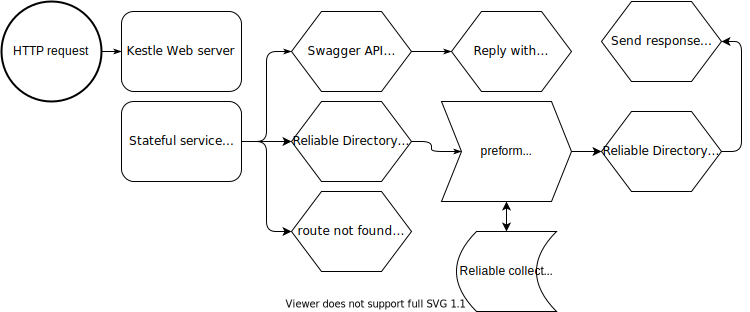
\includegraphics[scale=0.5]{images/Design_Stateful_service_1.0.drawio.png}

    This implementation contains 2 main codebases. The c\# dotnet web service that acts as a restAPI to the reliable collections using 3 controllers for the 2 default data structures implemented in the framework, and a Clojure codebase that contains the test suite as well as the API connector that handles parsing, connections and connections faults.

    \subsubsection{Infrastructure}
    The infrastructure in centered around v-net containing 6 Virtual machines all running linux, in this case ubuntu 18.04 and 20.04 for the jepsen host, I'll refer to the service fabric nodes from n1-n5 and the jepsen host as jepsenhost from now on.
    The 5 service fabric nodes are mostly self managing, applications can be deployed via either the Azure Service Fabric CLI\cite{https://docs.microsoft.com/en-us/azure/service-fabric/service-fabric-cli} or via visual studio\cite{https://docs.microsoft.com/en-us/azure/service-fabric/service-fabric-tutorial-deploy-app-to-party-cluster} which was the process used doing the development stages of the project.

    This Jepsenhost was management via ssh and rsync to deploy the newest version of the test code. Here a deployment pipeline could have been used to handle all of this by fetching, building and deploying via Jenkins or such a service but due to the goal of the project not being automated testing of Service Fabric, a bashcript instead used that deployed code, started applications, ran the test and retrieve results was used instead. rsync was used instead of scp to reduce the files being move back and Fourth from the deployment machine and the test cluster.

    The topology of the network is so that \\
    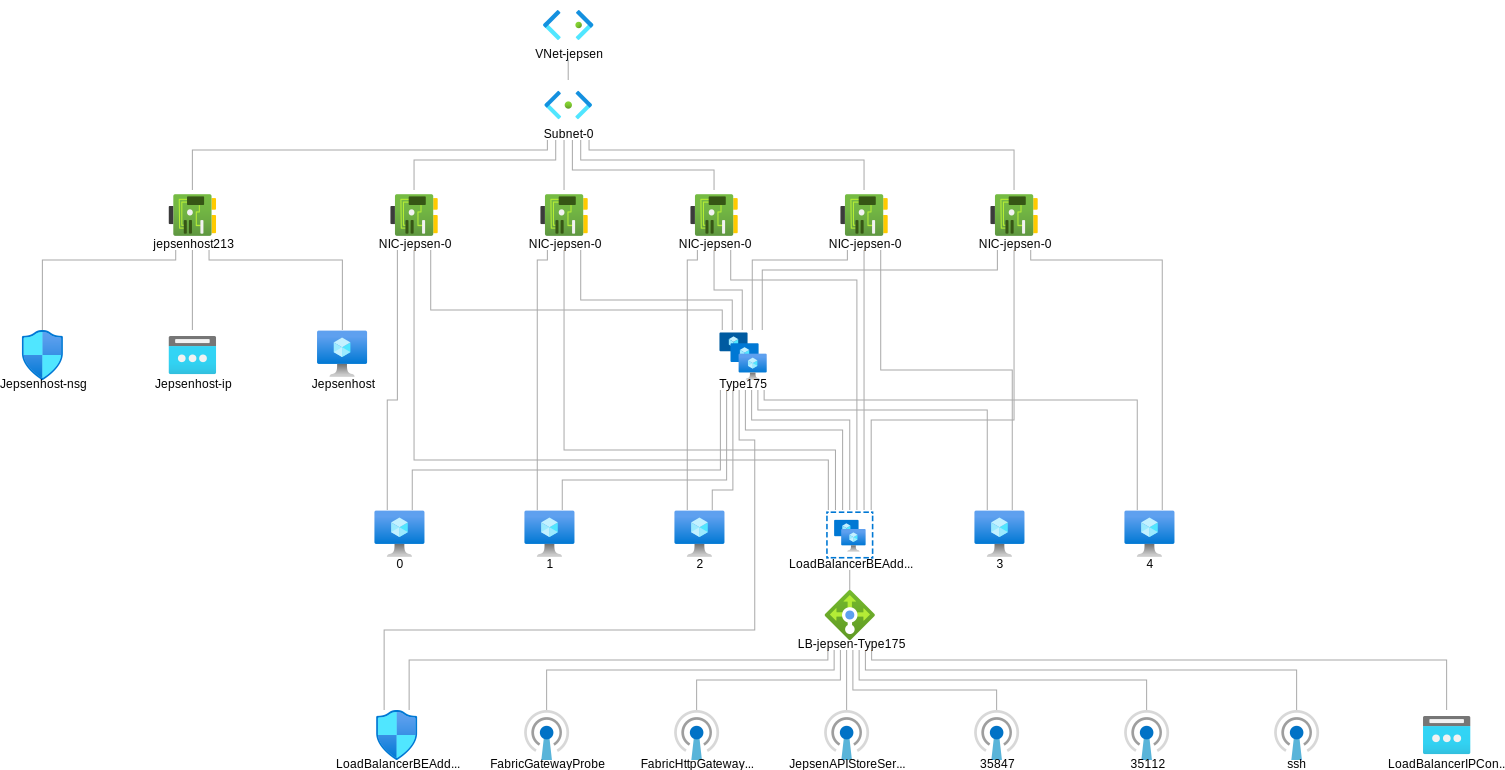
\includegraphics[scale=0.3]{images/topology.png}

    All traffic resides within the cluster and the load Balancer is only there for testing of the application and check if all endpoints work as expected.

    \paragraph*{Node Sizes}

    The initial node sizes were 2 cpu cores and 8 GBs of ram along with 20 GB local storage, as this was thought be enough to handle the workload of the test. This was later revised as the nodes had issues with disk space and often took a long time to setup and get ready for any given deployment, this was resolved by upgrading the size of the nodes to 4vcpu, 16GB ram and 80GB local storage per node. This configuration resulted in a much more well-behaved cluster. and this node size was kept for the reminder of the test. However the jepsenhost is slightly under-dimensioned compared to the workload it handles when computing on the result of the test. This is primary due to OOM errors that could be resolve with wither lowering the search space of the test or increasing the memory of the node itself.


    \section{Services}
    as mentioned earlier running these tests required multiple components, The stateful service that hosts the reliable collections from SF Reliability subsystem, a restless front-end that provides this data to clients via RESTAPI, a driver that handles the connection to this api and finally the Jepsen test suite itself consisting of both test suite and checker of the transactions and fault induced of the end system.

    \subsection{SF services}
    Using the 2 services approach as recommended from Microsoft provides multiple benefits but also a few negatives. the prime benefit it abstracting from the backend and adding a layer of validation, routing, and protection of the backend service. as well as greatly reducing the time that connections are held open to due RR times as all connections to the data store is kept within the cluster.

    \subsubsection{Stateful Reliable collection service}

    The stateful services provides 3 separate controllers that each provides one of the built in reliable collection types provided by service fabric. Reliable dictionary, reliable queue, and reliable concurrent queue. Fault handling is also handled at this stage where any fault stemming from the transactional issues is returned to the client via http status codes\cite{https://en.wikipedia.org/wiki/List_of_HTTP_status_codes}. eg node not primary, accepted, result not found.. etc.

    The fronted service simply provides these same apis but with wrappers and routing in case of a portioned design. This layer could also be used to built additional features but this was not the case as only the bare transactions supported by the reliable collections layer was needed.

    \subsection{Jepsen test suite}
    The Jepsen test suite contains many layers and two main components a connector that connects to the service fabric services, and the test suite itself.

    The drive is the simplest service that is based on a raft api that was completely rewritten to interact with the SF API along with a custom fault handler that is able to parse both the result that the reliable collections api provides along with with the http codes in case something doesn't behave as intended.

    The Jepsen test component contains 6 classes. a runner, a db class that prepares for the test, a client that interacts with the driver, nemesis that induces faults in the cluster and 3 workloads, queue, cqueue, and dict. testing the 3 separate types provided by service fabric.

    The runner type is the main class that handles defaults, cli input and test selection along with code that handles common behavior between the test. nemesis, db, along with other features that are mutual for all services that run in service fabric.

    the db class that is in charge for spinning up and tearing down the services along with functions for stating and stopping workers in the cluster.

    the nemesis class that contains the functions that kill, partition or otherwise mess and attempt to break the cluster.

    the 3 workloads.

    These each contain client for the test defining what endpoint to reach out to, a generator generating a sequence of transactions to preform on te database, and a checker that checks if our data stored behaved as expected.

    all types are expected to follow the repeatable-read consistently model. where the concurrent queue does best effort to meet the FIFO order of queued items compared the the normal queue following a FIFO ordering.

    \subsection{Implementation of the initial design.}

    The initial designed first targeted the reliable collection dict datatype. and presented a few issues with the design and implementation details that was not considered.

    The biggest hurdle here was developing code for the service fabric Linux cluster due to a non feature parity between it and the windows cluster which caused non favorable conditions such as no debugging, binary dump files that weren't readable by any tool available.

    Here a great amount of time was spent debugging, changing configuration files, stripping any unneeded libraries and rolling back to older versions of frameworks. it should be noted that the service fabric framework was kept at the newest release while .NET and similar aspects where rolled back to older releases.

    All of these attempts were however frugal, after spending newly 2 months deleting all code, starting from scratch using a different skeleton code. trying the implementations via java, going back to C\# getting a working solution on the windows service fabric implementation i reached out to Mikkel from Microsoft.

    The issue turned out to be 2 fold.
    \begin{itemize}
        \item .NET needing to be rolled back to 3.5
        \item the entry point having to be defined via .NET and the name of the DLL file. this was something i attempt prior by using a entry point.sh that did the same while his solution was just replacing where the windows version has .exe with .DLL and as a .NET entry point.
    \end{itemize}

    Finally i had a runnable version on Linux, or rather. i had a way to run my application on Linux as the issues didn't stop here. the Feature parity was still there. the dns service was still missing, this required a lot of endpoints to be hard coded, which induced as one active replica of a given service per node. eg we can only have 1 service running per node which would greatly reduce horizontal scaling of the partitions which would greatly increase the number of partitions required to handling greater workloads. running larger partitions on each node is also an option but from a performance, availability, and reliability it's much effect having lots of smaller nodes instead of one large database instance that require a lot of broadcasting to each partition replica.


    This required some changes to the design but was resolved by removing of the layers in the application and accessing the stateful service directly, or rather creating a parallel service in case the other services were required later.

    \subsubsection{Implementation details SF}
%TODO write section on Implementation details SF

    \subsubsection{Implementation details Clojure}
%TODO write section on Implementation details Clojure

    \subsection{2nd iteration of the design.}

    This 3rd service should simply provide the API directly from the stateful service, as the transactions are going to behave the same on a single partition as with 500 partitions. this 3rd service was configured such that replicas were active. this implies two things: Routing is no longer an issue, we need to route primary traffic to the primary node from our Clojure connector.

    this issue can be resolved in two ways. one is rather quick, while the other queries the SF cluster for which node is primary. the quick solution of just defining the primary at launch and from there checking which node allows writes in case the current node start blocking writes. this is a messy solution but as it doesn't induce noise in the data as these transactions are simply rejected/discarded it is therefor not an issue. optimally we should query the SF cluster for primary node, this implementation could chosen but as it takes more time and doesn't yield any further results this is deemed unnecessary.

    \subsection{Implementation of this design}


    The implementation of this interated design was supposed to have been been fairly streight forward however the non feature parity again poked it ungly head out again. The issues that arrived from here was mainly due to a change in the settings of the service fabric version which chaused some warnings to turn into errors. that exposed my inexperiance of working with the dotnet framework and the service fabric API. this issues were however eventually ironed out but a lot of times was lost due to the lack of debugging output from the cluster which turned the development cycle upside down as i had no way to execute the code without service fabric but the code wouldn't un on service fabric. The issue here ended up beging related to some changes in allowed port ranges that were allocatable to services and therefor killed the application as it was using an illigal port. these warnings were however not displayed correctly in the linux distribution.

    \subsubsection{Implementation details SF}
%TODO write section on Implementation details SF 2

    \subsubsection{Implementation details Clojure}
%TODO write section on Implementation details Clojure 2



    After this step the services to ready to test, as mentioned earlier in the paper 6 nodes are used to preform the test. 5 cluster member nodes and 1 jepsen test node.

    The steps to deploy and run the tests is as follows.

    \begin{enumerate}
        \item Deploy Cluster via a vm scaleset with a SF image, the jepsen host, a proximity group to prevent network issues, setup vlan and add the 6 servers, add a public IP to sasilirate connections to the test envoriment, Configure storage devices and firewalls to prevent undesired access and noise in the testing.
        \item Deploy the SF applications
        \item connent to the Jepsenhost server and sync test framework.
        \item run test framework with desired perameters
        \item pull test result to local machine to analyse results.
    \end{enumerate}

    For the first few rounds of testing everything went alright, however after running a few test exsamples

    \subsection{Issues}
%TODO write section on Issues
    Proximity group.

    Linux and windows versions being far from interchangeable and applications and services that function on windows/local machines fail crash on deployed cluster

    visual studio being unable to load .dmp files to debug crashed applications from the cloud.

    Visual studio remote debugger not working
%
%\subsubsection{Azure}
%
%Configuration issues
%
%Cluster becoming unhealthy/corrupt and nodes not being configured correctly after a reimage.
%
%
%\subsection{Jepsen Service}
%
%
%\section{Execution of the test}
%
%Steps.
%
%1 start Service Fabric cluster in azure.
%2. Add Jepsen node to Vlan of the cluster.
%3. Deploy SF application to the cluster. This is currently done via Visual studio but could also be automated from the jepson node.
%4. Deploy Jepsen code to the Jepsen node.
%5. Run Jepsen test.
%6. Retrive Test data from test node.
%5
%7. Clean up.

%


    \section{Results}

    \subsection{Introduction}

%TODO Write introduction to the results we've found
    What we results we have.

    \subsection{Rejected transactions}
    %TODO Write Rejected transactions
    We initially had a rejection rate of x
    ...

    Due to these reasons

    ...

    A revised setup was implemented to try and resolve this.

    ...

    Proximity group
    ...


    Proformance benefit.

    \subsection{Lost transactions}
%TODO Write Lost transactions

    \subsection{Violations of promised consistensy level}
%TODO Write Violations of promised consistensy level
    Intially violation but was maybe due to network queue or other network issues?


    \section{Discussion}

    %TODO write introduction

    \subsection{Deeper issue}

    %TODO Write Discussion Deeper issue
    The topic of understaning transactional models possibly stems for the teaching of database systems and a lack of understanding what the different consistency models define, what they allow and how they behave in practice,

    ....


    Going from this and other Jepsen tests on database it appears it's the issue is a board mislabling and misclassification of database sysetsms and what they can and can't do.
    ...
    Postgres replication and serisable,
    ...

    Mongo db dropping data
    ...

    Casandra last-write wins, issues, and a attempt at a solution via Atomic clocks
    ...

    Elatic search issues.
    ...

    Some of the implications this can have on real world usecases,

    ...

    how to resolve these issues that arrise from mislabled and misunder consistency models.

    ...

    Enable better understanding of databases, transaction models, and usecases doing teaching of database courses where behavoir is better explained, This should not in depth but just to the level of read uncommitted or last-write-wins databases are fine for logging but should be avoided for most systems as they have a lot of uninteded behavoir, or at least theses systems should be below other layers that ensure that the data is persistent before a commit is accepted.

    ... should maybe be defined as future work.

    Whats next, Defining a standard for testing and certifying database systems towards transactional model that allows the industry to standardize the labling and allows user and developers to choose the current system for their usecase and avoid the headaces of phatom behavoir.

    this could be done via automated testing and verifycation of a given system in it's different transactional configureations.


    \chapter{Conclusion and Outlook}
    \section*{Conclusion}
 %TODO write Conclusion

    \section*{Outlook}
%TODO write Outlook


    \section{Future Work}
%TODO write Future Work
    Future work could include implementing a deeper testing suite that checks for more types of invariants and issues that might occur in the system.





    \newpage


    \chapter{Appendix}

    \pagestyle{empty}
    \printbibliography


    \section{Proposal}
    \input{Proposal}


    \section{Schedule}

% Please add the following required packages to your document preamble:
% \usepackage{multirow}
% \usepackage[table,xcdraw]{xcolor}
% If you use beamer only pass "xcolor=table" option, i.e. \documentclass[xcolor=table]{beamer}

    \begin{tabular}{clll}
        \multicolumn{2}{l}{Mark Jervelund thesis plan} & & \\
        & Week 45 &                                                    &                                                                                      \\
        & Week 46 &                                                    & \multirow{-2}{*}{\text{Study Jensen test}}                                           \\
        & Week 47 &                                                    &                                                                                      \\
        \multirow{-4}{*}{November} & Week 48 &                                                    & \multirow{-2}{*}{\text{Finish study on Jepsen test}}                                 \\
        & Week 49 &                                                    &                                                                                      \\
        & Week 50 &                                                    & \multirow{-2}{*}{\text{Study Service Fabric} }                                       \\
        & Week 51 &                                                    &                                                                                      \\
        & Week 52 &                                                    & \multirow{-2}{*}{\text{Christmas break}}                                             \\
        \multirow{-5}{*}{December} & Week 53 &                                                    &                                                                                      \\
        & week 01 & \multirow{-10}{*}{\text{Structured study 8 weeks}} & \multirow{-2}{*}{\text{Finish Study Service Fabric} }                                \\
        & Week 02 &                                                    &                                                                                      \\
        & Week 03 &                                                    & \multirow{-2}{*}{\text{designing the experiment}}                                    \\
        \multirow{-4}{*}{January}  & Week 04 &                                                    &                                                                                      \\
        & Week 05 &                                                    & \multirow{-2}{*}{\text{designing the experiment} }                                   \\
        & Week 06 &                                                    &                                                                                      \\
        & Week 07 &                                                    & \multirow{-2}{*}{\text{Execute the experiment}  }                                      \\
        \multirow{-4}{*}{February} & Week 08 &                                                    &                                                                                      \\
        & Week 09 &                                                    & \multirow{-2}{*}{\text{Analyse the experiment}}                                      \\
        & Week 10 &                                                    &                                                                                      \\
        & Week 11 & \multirow{-10}{*}{\text{Experiment 10 weeks}}      & \multirow{-2}{*}{\text{discover what the findings from the experiment is}}           \\
        & Week 12 &                                                    &                                                                                      \\
        \multirow{-5}{*}{March}    & Week 13 &                                                    & \multirow{-2}{*}{\text{Running additional experiments if needed Full on write mode}} \\
        & Week 14 &                                                    &                                                                                      \\
        & Week 15 &                                                    & \multirow{-2}{*}{\text{Full on write mode} }                                         \\
        & Week 16 &                                                    &                                                                                      \\
        \multirow{-4}{*}{April}    & Week 17 &                                                    & \multirow{-2}{*}{\text{Full on write mode} }                                         \\
        & Week 18 &                                                    &                                                                                      \\
        & Week 19 &                                                    & \multirow{-2}{*}{\text{Full on write mode Send out thesis for feedback}}             \\
        & Week 20 &                                                    &                                                                                      \\
        & Week 21 & \multirow{-10}{*}{\text{Thesis writing 10 weeks}}  & \multirow{-2}{*}{\text{Correction} }                                                 \\
        \multirow{-5}{*}{May}      & Week 22 &                                                    &                                                                                      \\
        & Week 23 & \multirow{-2}{*}{\text{goal}}                      & \multirow{-2}{*}{\text{Hand in}}                                                     \\
        & Week 24 & \multicolumn{1}{l}{}                               & \multicolumn{1}{l}{}                                                                 \\
        & Week 25 & \multicolumn{1}{l}{}                               & \multicolumn{1}{l}{}                                                                 \\
        & Week 26 & \multicolumn{1}{l}{}                               & \multicolumn{1}{l}{}                                                                 \\
        \multirow{-5}{*}{June}     & Week 27 & \multicolumn{1}{l}{}                               & \multicolumn{1}{l}{}                                                                 \\
        \multicolumn{1}{l}{}       & Week 28 & \multicolumn{1}{l}{}                               & \multicolumn{1}{l}{}                                                                 \\
        \multicolumn{1}{l}{}       & Week 29 & \multicolumn{1}{l}{}                               & \multicolumn{1}{l}{}                                                                 \\
        \multicolumn{1}{l}{}       & Week 30 & \multicolumn{1}{l}{}                               & \multicolumn{1}{l}{}                                                                 \\
        \multicolumn{1}{l}{}       & Week 31 & \multicolumn{1}{l}{}                               & \multicolumn{1}{l}{}
    \end{tabular}

\end{document}





